\chapter{Introduction}
\label{chap:intro}

% First, standard motivation
  % 0    Ultimately, explanations for complex models require some sort of generation
  % 1    technique. On thing to generate is heatmaps, another is class-maximizing
  % 2    samples, while a third is counterfactuals. Most previous work has tried to
  % 3    use established classification networks to generate explanations.  In this
  % 4    thesis, a different approach is taken. With the increased popularity of
  % 5    generative models such as GANs,  VAEs, Normalizing Flows, Transformers,
  % 6    etc., it seems natural to use such networks as a starting points for
  % 7    generating explanations. This thesis lies in the intersection of generative models
  % 8    and explainabilty. As such, it contributes both to the field of generative
  % 9    models, in particular Normalizing Flows and Image synthesis evaluation; and to
 % 10    the field of explainability.

\section{Challenges}\label{sec:challenges}
\content{Give short introduction to what this section is supposed to do.}

\paragraph{Improving Generative Models.}
\frederik{I am not sure that this challenge is conveyed properly. Maybe try, before even reading it, to take a step back and take a note of the four things the we want to say in this paragraph.}
% When Normalizing Flows perform well enough, they could replace regular CNNs for classification as well. 
From the general idea that an explanation requires the generation of new evidence, we see an immediate challenge in improving the generative capabilities of deep neural networks.
\frederik{Make sure to phrase the fundamental idea the same way every time.}
The generative necessity is also present in humans.
For example, had a human not been able to imagine (generate) a situation in which she would have made an alternative decision, then she would not be able to explain her decision by an alternative either.
We believe that when generative performance of deep neural networks is improved, it will open many doors for how such networks can be explained.

\begin{enumerate}
    \item Qualify
    \item Expressiveness
    \item Speed
    \item Evaluation
\end{enumerate}

\paragraph{Explaining Deep Neural Network}
Most related work to this thesis either consider generative performance, predictive performance, or explainability in an isolated manner. 
Each discipline is gaining much traction and demonstrates outstanding performance.
Unfortunately, only rarely are the disciplines crossed. 
It is a great challenge to combine the disciplines to get deep models that have high performance on predictive performance while being able to generate high-quality explanations.

\begin{enumerate}
    \item Explanations that convey truthful and interpretable recourses
    \item Join forces between generative models and explainability
    \item Evaluation
\end{enumerate}

\section{Contributions}\label{sec:contributions}
\content{Describe how our work fit into the picture described above.} 
\paragraph{Improving Generative Models.} 
This thesis makes a three-fold contribution to this first challenge. 
First, we present work on how to efficiently parameterize weight matrices of neural networks in their Singular Value Decomposition (SVD), which is beneficial for Normalizing Flows (\paperref{pap:svd}). 
Having direct access to the singular values enables efficient manipulation of condition number, computation of determinants, and inverse computations, to name but a few.
Second, we demonstrate that, when chosen by a neural network, a single reflection is theoretically as expressive as any number of reflections (\paperref{pap:refl}).
We call such reflections Auxiliary reflections.
Auxillary reflections can be used as a new type of layer in Normalizing Flows, but they also have applications in recurrent neural networks, where orthogonal transformations help mitigating exploding and vanishing gradients. 
Third, we introduce FastFID; an algorithm that allows backpropagating through the FID score efficiently (\paperref{pap:fastfid}). 
Prior to our work, training generative models with FID was practically infeasible.
In practice, FastFID reduces computation time up to $500\times$, when the mini-batch size is sufficiently small. 
The algorithm potentially allows training even better Normalizing Flows or any other generative model.

\paragraph{Explaining Deep Neural Networks.}
In this thesis, we make the connection between invertible Neural Networks and the area of explainability.
In particular, we introduce ECINN which is an algorithm for computing counterfactual explanations efficiently (\paperref{pap:ecinn}).
The algorithm utilized generative capabilities of invertible neural networks to produce high-quality explanations by correcting input data in a latent space.
The method is up to $1000\times$ faster than gradient based methods.

\todo{Write paragraph on evaluating counterfactual explanations.}

\section{Outline}\label{sec:outline}
\content{
    Outline of the rest of the thesis.
}
% % % % % % % % % % % % % % % % % % % % % % % % % % % % % % % %
% DEEP GENERATIVE MODELS                                      %
% % % % % % % % % % % % % % % % % % % % % % % % % % % % % % % %
% Notes on VAE http://ruishu.io/2018/03/14/vae/
\chapter{Deep Generative Models}\label{chap:flows}
\section{Introduction} 

\content{ Introduction to generative models. Talk about VAEs and GANs as approximate likelihood and then present Autoregressive models and Normalizing Flows as exact likelihood models. } 

Deep learning models have had immense success during the last decade \cite{alexnet, noisyStudent, resnet, vae, gans}. 
Initially, deep learning models were used for supervised tasks, like image classification \cite{alexnet}.
In some cases, even surpassing human performance~\cite{noisyStudent}.
As an unsupervised learning approach, deep generative models have become increasingly popular since 2014 with the introduction of, e.g., Generative Adversarial Networks (GANs)\cite{gans}, Variational Auto-encoders (VAEs) \cite{vae}, and Normalizing Flows (NFs) \cite{nice, rezende2015variational}; three different paradigms for modelling data distributions to achieve efficient unconditional sampling.

Generative models are of particular interest to this thesis because the ability to generate ``synthetic'' data from neural networks is strongly tied to explaining neural networks.
As such, mastering generative abilities potentially opens up for generating better explanations.
For example, 
\todo{continue here, something about using a generative model to explain another model from synthesized data.}
% This could also be the paper on explaining with ibinn. They use properties of inns to visualize decision boundaries, display trade-offs between classification and generation capabilities, etc.
% However, we will describe this paper further below...

% \content{ Emphasize why we focus on invertible neural networks - surjectiveness. }
In the present work, we find NFs to be of particular interest because of their bijective nature. 
For any \emph{output} of an NFs, there is exactly one \emph{input}.
Bijectivity thus potentially disambiguates solutions to explainability-related problems.
In contrast, VAEs are constructed to produce embeddings of lower dimensionality, which in turn yields surjective models. 
The lack of bijectivity makes it ambiguous which exact input belongs to an internal representation, which makes such representations harder to analyze.

In this section, we describe NFs, some of their issues, and how we contribute to improving them. 


\section{Normalizing Flows}\label{sec:nf}
\content{Change of variables formula + variational dequantization. }
\content{Layers and architectures - What are the missing pieces and how did we contribute. }
% \content{Additional tricks. Here I am thinking \textsc{flow++} and the like. }
% \content{\textbf{Applications} \frederik{I actually don't really know anything about this. However, I think that it will make a very nice bridge to how explanations could potentially be used.} } 

\content{
    Describe how \emph{Fast SVDs in Neural Networks} fins in and solves problems. 
    \begin{itemize}
        \item Fast (compare to LU and QR decompositions of previous work)
        \item Orthogonality and analysis of singular values
        \item Other benefits and applications (spectral normalization, rnns, etc.)
    \end{itemize}
}

% I think that I will drop this one
% \content{
    % One Reflection Suffice is a follow up, which utilize the orthogonal property of reflections and make them learnable.
    % This allows more flexible normalizing flows and allows adding more parameters to the network (similar to coupling layers).
% }


\content{ Conditional Normalizing flows }
What are the approaches and why are they interesting.
\todo{should we somehow move this to where we discuss ECINN?}
\content{
    This actually relates very closely to ECINN by theoretically belongs to normalizing flows.
    We need to describe and maybe demonstrate how, e.g., $\beta$-values trades off generative and predictive performance.
    We could also describe more in detail what is presented in \cite{expl-inn}  about how such classifiers become more interpretable. 
}

\section{Evaluating Generative Models}\label{sec:rw-eval}
\content{Convince people that it is hard to validate high-dim generative models. Tell how there are many metrics and that none of them captures the whole picture. I think that this is actually also a good motivation for the current paper.}

\content{ 
    Fr\'eche inception distance. Give an intuition about what it is, why it was traditionally slow to compute and how it can become faster and suddenly be used. 
    I think that some of the intuitions with why it is okay to use batches also deserves some space here. This was not included in the paper while discussed in the rebutal. 
}


% % % % % % % % % % % % % % % % % % % % % % % % % % % % % % % %
% EXPLAINING DEEP NEURAL NETWORKS                             %
% % % % % % % % % % % % % % % % % % % % % % % % % % % % % % % %
\chapter{Explaining Deep Neural Networks}\label{chap:rw-counterfactuals}

\content{Give the broughter perspective}

\section{Introduction}\label{sec:attributions}
\content{
    \begin{itemize}
        \item Illustrateive example of why this is hard and what one might want from an explanation. 
        \item Give the broader overview: surrogate (transparant) models,  Attribution techniques, counterfactual examples, etc.
    \end{itemize}
}

\section{Counterfactual Explanations}
\label{sec:counterfactuals}
\paragraph{The Ideal World}
\content{ Causal structural models, where we can marginalize probablities. }

\paragraph{When Shit gets deep}
\content{
    In deep neural networks, it is generarally unknown how to make stuctural causal models without intervantional data \cite{Verma2020}.
    So for now, we need to do with less. 
}

\content{
    Describe the overall view of approaches and put ECINN into perspective.
}

\content{
    If we get one of the authors of the FACE paper \cite{Poyiadzi2020} on the committee, it would be really nice to further describe the relationship between ECINN and feasibility of the counterfactuals generated.
    I believe that we can relatively easily compute feasibility of counterfactuals from  Reinmann sums.
    See notes in Mendeley.
    There are no ``feasibility values'' reported in their paper but the relation would still be fun to make. We can maybe even compare by computing them for FACE ourself.
}

\content{
    Another idea is to extend ECINN with restrictions on the counterfactuals by imposing an optimization constriant.\\
    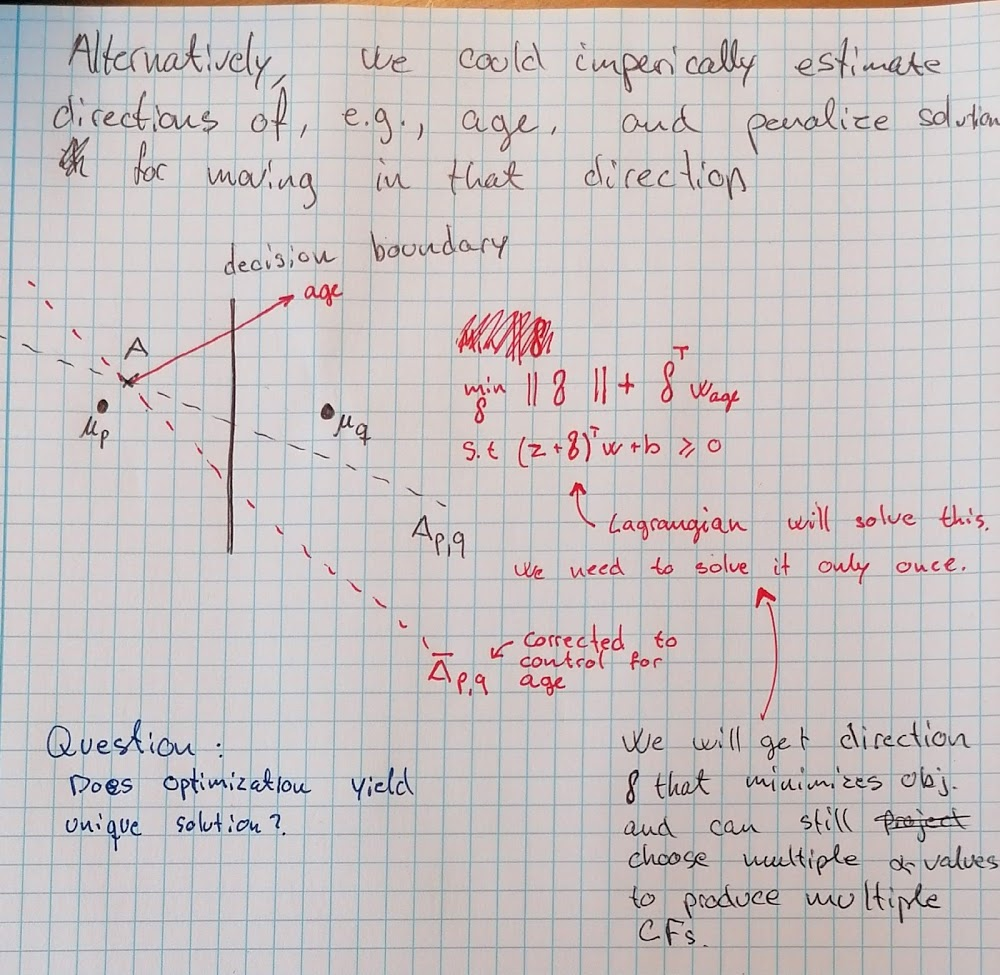
\includegraphics[width=0.9\textwidth]{graphics/IMG_20210623_113433.jpg}
}

\section{Evaluating Explanations}

\content{ 
    Initial description with general idea about why this is so hard. 
    The problem is that we cannot even come up with an example, where we know the answer. We can make proxies but not the true story.
} 

\paragraph{Ideas from Heatmaps}
\content{ 
    \begin{itemize}
        \item AOPC
        \item Qualitative
        \item I really need to find example with FakeMNIST again!!
    \end{itemize}
}

\paragraph{Counterfactual evaluations}
\content{
    \begin{itemize}
        \item Start by relating to motivating example in the introduction of the section.
        \item Describe similar issues for counterfactual explanations.
        \item Put Evaluation paper into context and STRESS that there is a huge need for a standardized test for counterfactual methods
        \item Describe how we try to provide this with the evaluation paper. 
    \end{itemize}
%    
}

\content{
    \cite{Laugel2019} also talks about justification of counterfactuals, in which CFs must be connected by a path to a real point of the target class, such that every point on the path is also from that class.
    We have this by construction with ECINN and should report this in the thesis.
}

\chapter{Conclusion} 
% \todo{ Sum up: }
% \section{Discussion}
Discuss how 

% \section{Conclusion}

% \section{Future Work}

Describe open problems / future directions. 
Given introduces tools how to move forward on open problems given my thesis. 





% % % % % % % % % % % % % 
%  Figures form simple encoder / decoder test. 
\begin{figure}
    \centering
    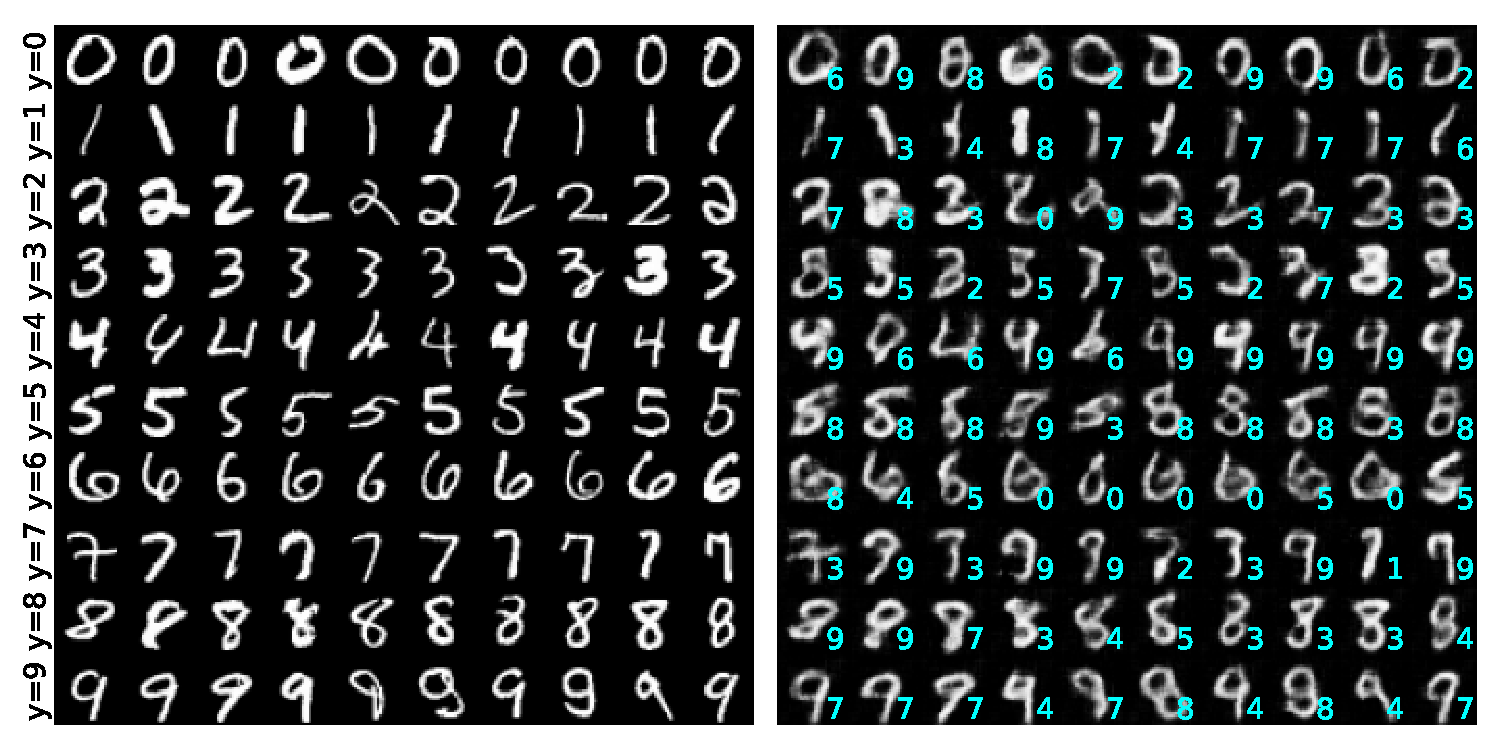
\includegraphics[width=\textwidth]{graphics/image_optimization.pdf}
    \caption{Caption}
    \label{fig:my_label}
\end{figure}
\begin{figure}
    \centering
    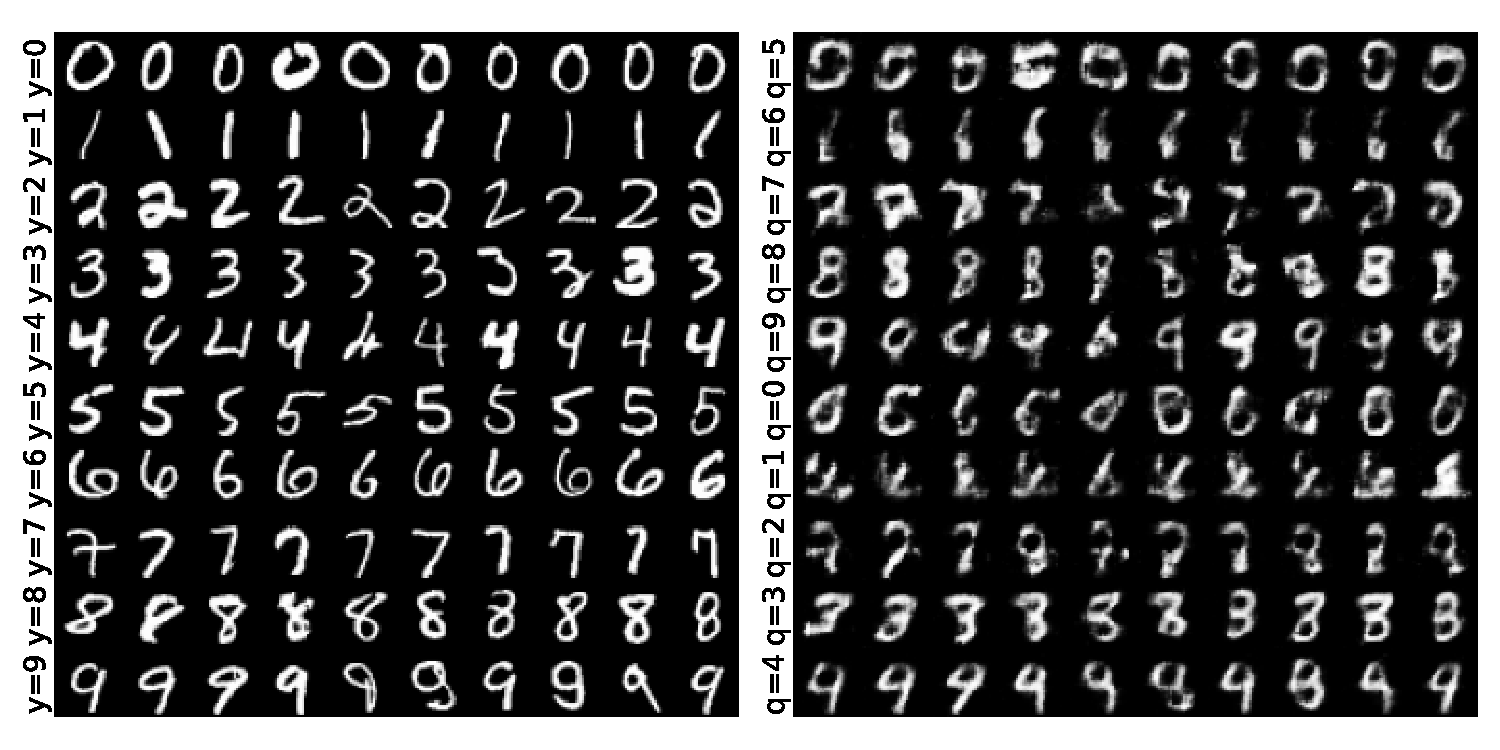
\includegraphics[width=\textwidth]{graphics/decoder_optimization.pdf}
    \caption{Caption}
    \label{fig:my_label}
\end{figure}